\chapter{Particionado y sistemas de ficheros}
Anteriormente hemos visto que los \hyperlink{dispositivos_almacenamiento}{sistemas de almacenamiento} (más conocidos como discos duros) son dispositivos que pueden ser de distintos tipos, capacidades, tamaños...

A la hora de usar un disco duro en nuestro Sistema Operativo, tenemos que tener en cuenta al menos dos cosas:

\begin{itemize}
    \item \textbf{Tipo de particionado}.
    \item \textbf{Sistema de ficheros}.
\end{itemize}

Dependiendo del Sistema Operativo, y el modo que elijamos durante la instalación, nos dará más opciones o menos a la hora de elegir, modificar o personalizar algunas de estas opciones.

Para tomar las decisiones correctas, deberíamos conocer, al menos, los siguientes detalles:

\begin{itemize}
    \item Número de discos duros instalados en el equipo.
    \item El tipo de cada uno (mecánico, SSD, NVMe...).
    \item Tamaño de los mismos.
    \item Función que va a realizar el equipo.
\end{itemize}

De esta manera, podremos realizar un análisis previo de cómo queremos realizar la instalación.


\section{Particionado MBR y GPT }
Los discos duros se dividen en lo que se llaman particiones. Es una manera de realizar divisiones lógicas del espacio, que actúan de forma independiente entre sí.

\textbf{El símil del particionado de disco duro es un armario}: tenemos una cantidad de hueco posible, que decidimos “particionar” añadiendo estanterías tanto horizontales como verticales, donde almacenar distintos tipos de ropa, de manera independiente, en cada uno de esos compartimentos.

A la hora de crear la tabla de particiones de un disco duro podemos elegir entre los siguientes tipos:

\begin{itemize}
    \item \textbf{MBR}: De \textit{Master Boot Record}, o también conocido como \textbf{tabla de particiones DOS}.
    \item \textbf{GPT}: De \textit{GUID Partition Table}, propuesta por la especificación EFI, más moderna que la anterior.
\end{itemize}

En la siguiente tabla se pueden identificar algunas de las diferencias más destacadas entre ambos sistemas:

\begin{yukitblrcol}{XXX}
    & MBR & GPT\\
    Tamaño máximo de partición & 2 TB & 18 Exabytes \\
    Nº de particiones primarias & 4 & Ilimitado

    (Windows reconoce 128)\\
    Tabla de particiones& Al inicio & Al inicio y al final (backup) \\
    ID de la partición & Se almacena en la partición & Identificador único de GUID\\
    Soporte de arranque múltiple & Débil & Las entradas del gestor de arranque están en una partición separada  \\
\end{yukitblrcol}

Para comprobar cuál es el sistema de particiones de nuestro disco duro lo podemos hacer desde:
\begin{itemize}
    \item En \textbf{Windows}: Desde el administrador de discos duros.
    \item En \textbf{GNU/Linux}: Con GParted, fdisk, ...
\end{itemize}

A continuación se pueden ver capturas de pantalla de distintos discos en un equipo Windows.


\begin{minipage}{0.45\linewidth}
    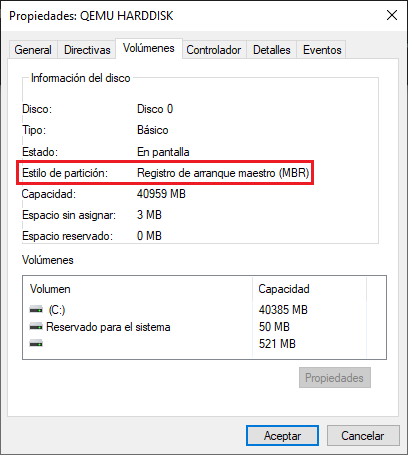
\includegraphics[frame,width=\linewidth]{hdd_mbr.png}
\end{minipage}
\hfill
\begin{minipage}{0.45\linewidth}
    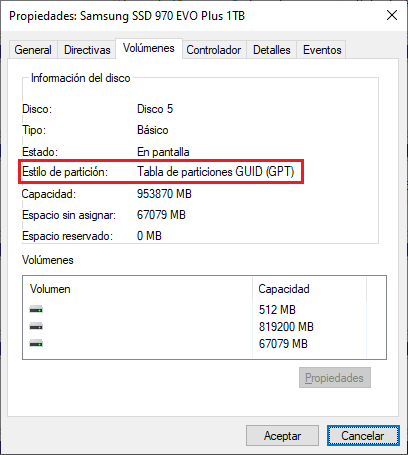
\includegraphics[frame,width=\linewidth]{hdd_gpt.png}
\end{minipage}


\section{RAID}

RAID (en inglés \textit{redundant array of independent disks}) es un grupo o matriz redundante de discos independientes que hace referencia a un sistema para crear una unidad de almacenamiento lógica utilizando varias unidades de almacenamiento. De esta manera, \textbf{el sistema operativo sólo ve un único almacenamiento lógico, que “por detrás” utiliza varios}.

Dependiendo del tipo de grupo creado, los datos se distribuirán o se replicarán entre las unidades que forman el grupo.

A la hora de crear un sistema RAID, podemos hacerlo de dos maneras:
\begin{itemize}
    \item \textbf{RAID por hardware}: Existe un hardware especializado que se encarga de realizar las operaciones del sistema RAID, así como de crearlo, gestionarlo, hacer las operaciones de paridad necesarias... Podemos diferenciar dos sub-tipos:

    \begin{itemize}
        \item \textbf{Placa Base}: Algunas placas base tienen un controlador especializado que se encarga de la creación del RAID, que se puede gestionar desde el sistema UEFI.
        \item \textbf{Tarjeta controladora especializada}: Este sistema es el \textbf{más profesional}. Los discos duros en lugar de ir conectados a la placa base, se conectan a esta tarjeta (normalmente a través de unos cables especiales que se conectan por SATA al disco duro y mediante conectores especiales a la tarjeta). Hay veces que cuentan con una batería propia (para controlar la escritura en caso de que el servidor se quede sin alimentación) y con un menú propio de configuración.
    \end{itemize}

    \item \textbf{RAID por software}: El Sistema Operativo se encarga de crear y gestionar el sistema RAID. En caso de necesitar realizar paridad, la CPU se encargará de ello, quitando recursos a otros procesos.
\end{itemize}

Tal como se puede ver en la \href{https://es.wikipedia.org/wiki/RAID}{Wikipedia}, existen distintos tipos de RAID, que también pueden combinarse entre sí, pero a continuación se explicarán los más estándares.

\subsection{RAID 0}

\begin{minipage}{0.63\linewidth}
    \setlength{\parskip}{1.2em}

    Un sistema RAID 0 distribuye los datos de manera equitativa entre dos o más discos, sin hacer uso de información de paridad. RAID 0 \textbf{no habilita redundancia}, por lo que \textbf{si uno de los discos duros del sistema se estropea, se perderán todos los datos}.

    \textbf{Espacio total = sumatorio del espacio de los discos.}

    Con este sistema se puede conseguir una mayor velocidad de escritura, ya que los datos se escriben de manera simultánea en todos los discos.


\end{minipage}
\hfill
\begin{minipage}{0.28\linewidth}
    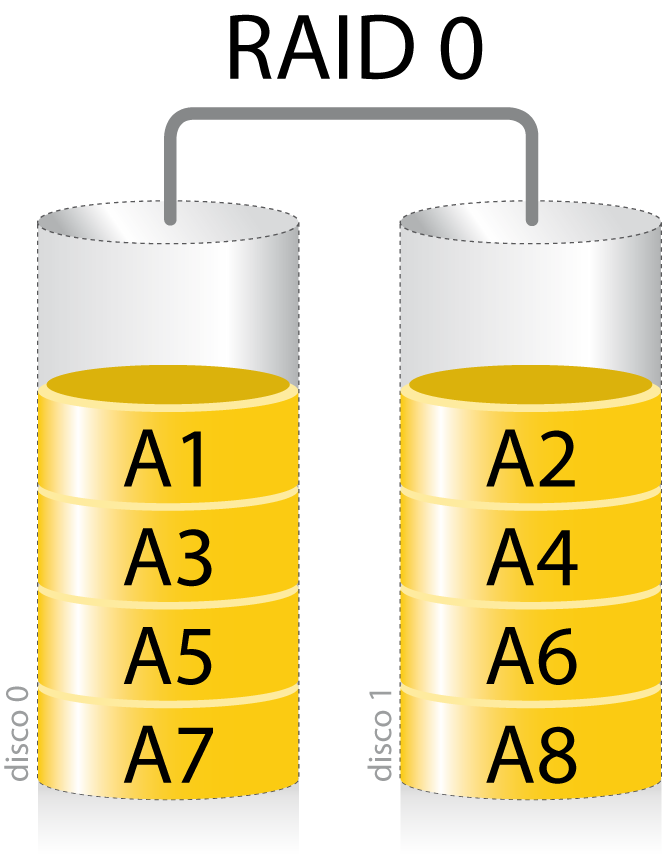
\includegraphics[width=\linewidth]{Raid0.png}
    \vspace{-30pt}
    \captionof{figure}{Fuente: \href{https://commons.wikimedia.org/wiki/File\:Raid0.png}{Wikipedia}}
\end{minipage}

\errorbox{
    \begin{center}
        \textbf{No se aconseja utilizar RAID 0 en sistemas con datos importantes.}
    \end{center}
}

\vspace{10pt}
\subsection{RAID 1}
\begin{minipage}{0.63\linewidth}
    \setlength{\parskip}{1.2em}
El RAID 1, también conocido como RAID espejo, crea una copia exacta de los datos en dos o más sistemas de almacenamiento.

Resulta útil cuando queremos tener seguridad a la hora de preservar los datos a pesar de no aprovechar la capacidad total del conjunto de los discos. \textbf{Si uno de los discos falla, los datos no se pierden}.

\textbf{El RAID 1 sólo puede ser tan grande como el más pequeño de los discos.}

No se mejora el rendimiento en escritura, pero en la lectura el tiempo se reduce al poder usar varios discos de forma simultánea.
\end{minipage}
\hfill
\begin{minipage}{0.28\linewidth}
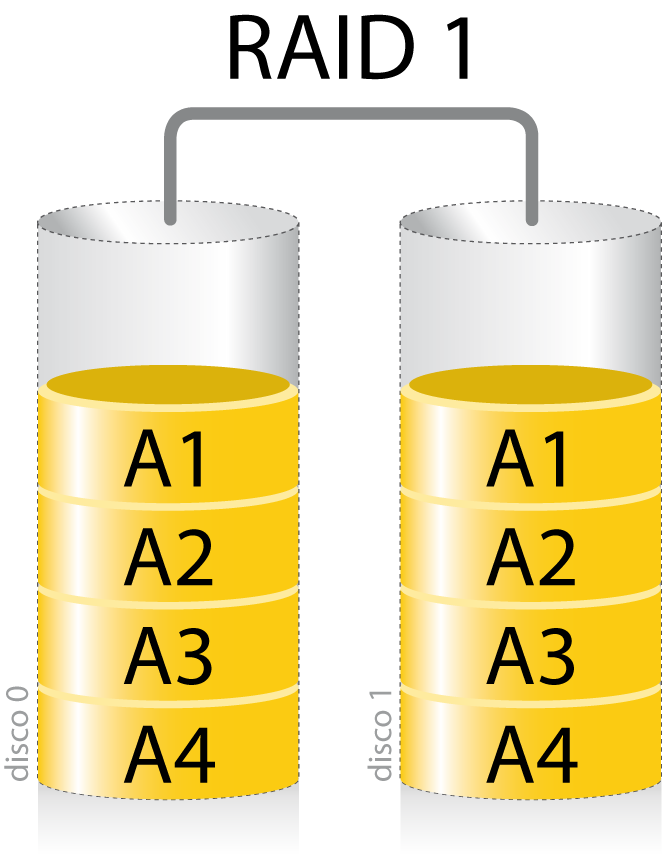
\includegraphics[width=\linewidth]{Raid1.png}
\vspace{-30pt}
\captionof{figure}{Fuente: \href{https://commons.wikimedia.org/wiki/File\:Raid1.png}{Wikipedia}}
\end{minipage}


\subsection{RAID 5}

RAID 5 es una división de los datos a nivel de bloques que distribuye la información entre el conjunto de discos que lo forman, y añadiendo \textbf{paridad}. La paridad se utiliza para poder corregir errores o generar los datos en caso de pérdida de uno de los discos.

Para crear un sistema RAID 5 se necesitan al menos 3 discos duros, quedando uno de ellos “inutilizado” en lo que se refiere a guardar información.

\textbf{El volumen total = (n-1)*tamaño de disco más pequeña}, donde “n” es el número de discos que forman el RAID 5. Si tenemos 3 discos de 2TB, el tamaño total será = (3-1)*2TB = 4TB.

En caso de rotura de un disco duro, los datos se mantienen, pero el sistema RAID 5 no soportaría la rotura de un segundo disco duro. Es por ello que cuando sucede esto, hay que sustituir el disco dañado para que se regeneren los datos en el nuevo disco duro, gracias al sistema de paridad.

\begin{center}
    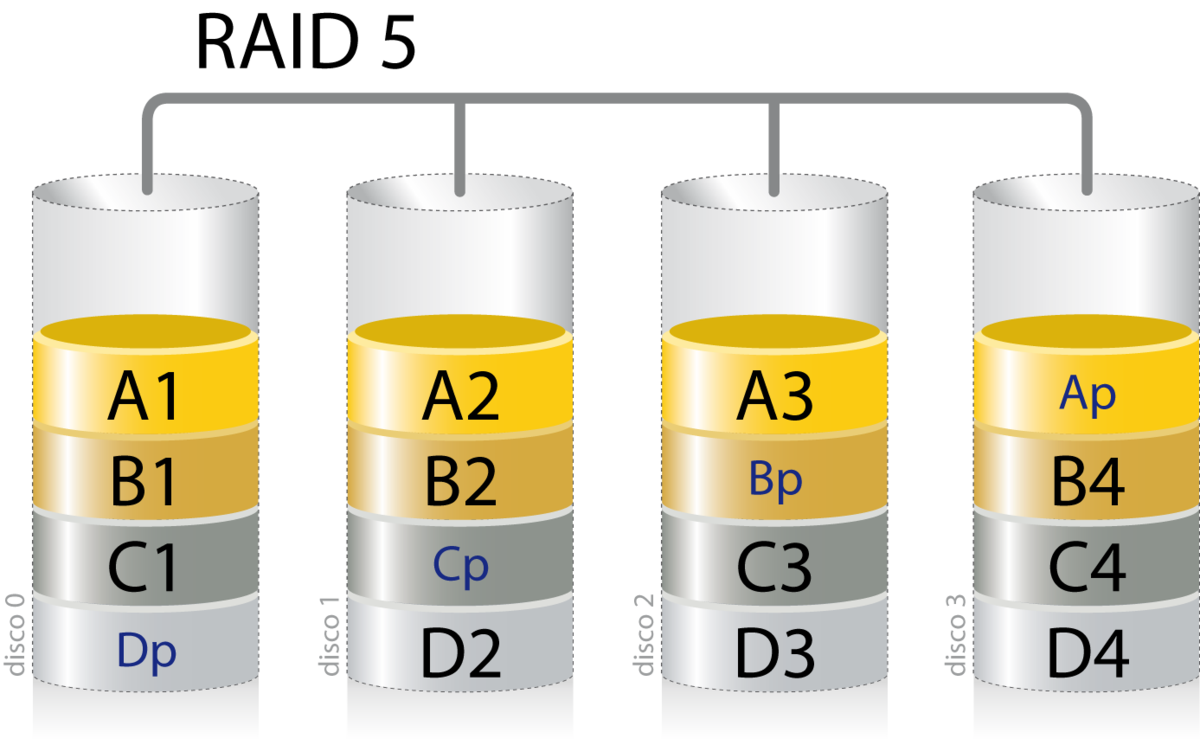
\includegraphics[width=0.5\linewidth]{Raid5.png}
    \vspace{-15pt}
    \captionof{figure}{Fuente: \href{https://commons.wikimedia.org/wiki/File\:Raid5.png}{Wikipedia}}
\end{center}

\subsubsection{Discos spare/reserva}

Existen variantes de RAID 5, y algunas controladoras hardware también implementan, la posibilidad de tener discos denominados “\textbf{\textit{hot spare}}”, o \textbf{de reserva}.

Estos discos están conectados (a la controladora, o la placa base) pero sin estar dentro del grupo RAID. Entrarán a formar parte del grupo en el momento en el sistema detecte que uno de los discos pertenecientes al grupo está fallando, y por tanto el sistema RAID esté degradado.

De esta manera, al entrar en el grupo, el RAID comenzará a arreglarse de manera automática sin tener que esperar a que el administrador de sistemas se entere de que ha habido algún error.


\section{Sistemas de ficheros}
\textbf{Los sistemas de ficheros controlan cómo se almacenan y recuperan los datos}. Sin un sistema de archivos, los datos colocados en un medio de almacenamiento serían un gran cuerpo de datos sin manera de saber dónde termina un dato y comienza el siguiente.

\infobox{\textbf{Un sistema de ficheros nos proporciona una “\textit{vista lógica}” de cómo se almacenan los datos.}}

Las funciones principales de los sistemas de ficheros son:

\begin{itemize}
    \item Asignar espacio a los archivos.
    \item Administrar el espacio libre (reorganizándolo en caso necesario).
    \item Provee una API a los programas para crear, borrar, modificar y cerrar los ficheros.
    \item Permite gestionar el acceso a los ficheros (permisos de ficheros).
    \item Optimizar el rendimiento de acceso.
\end{itemize}


\subsection{Ficheros}
Un fichero (o archivo) es una secuencia de bytes almacenado en un dispositivo que \textbf{es identificado por un nombre y normalmente una extensión}. Los ficheros pueden ser almacenados en directorios, y estos a su vez en otros directorios.

En inglés sí existe distinción entre \textbf{\textit{file}} y \textbf{\textit{archive}} siendo la diferencia:

\begin{itemize}
    \item \textbf{File}: Es un conjunto de información que se almacena de manera conjunta. Cómo se almacena esa información depende de cómo se ha diseñado el programa que lee y/o escribe esa información.
    \item \textbf{Archive}: Un archivo es un conjunto de ficheros almacenados junto con \textit{\textbf{metadata}} (datos que aportan información sobre datos). El ejemplo más claro puede ser un archivo comprimido, archivos que permiten distribuir programas, ...
\end{itemize}

Los ficheros cuentan con un nombre para que los podamos identificar. Dependiendo del sistema de ficheros puede ser:
\begin{itemize}
    \item \textbf{Case sensitive}: O sensible a mayúsculas/minúsculas. Esto quiere decir que “hola.txt” y “HOla.txt” son dos ficheros distintos.
    \item \textbf{Case insensitive}: O insensible a mayúsculas/minúsculas. No puede haber dos ficheros con las mismas letras en el mismo orden, aunque sean mayúsculas y minúsculas. “hola.txt” y “HOla.txt” no pueden convivir en el mismo directorio.
\end{itemize}

Los ficheros suelen contar con una \textbf{extensión}, que va después del nombre seguido de un punto, y normalmente suele ser de 3 letras para la mayoría de casos. Estas extensiones sirven para conocer el tipo de fichero a simple vista, pero no determina el contenido del fichero.

\warnbox{\textbf{La extensión no determina el tipo de fichero que es. Si renombramos un fichero con una extensión, el contenido del fichero sigue siendo el mismo}}

Un pequeño listado de  \href{https://en.wikipedia.org/wiki/List_of_filename_extensions}{extensiones}  habituales que podemos identificar:

\begin{itemize}
    \item \textbf{Documentos de texto y ofimáticos}: .txt, .doc, .docx, .xls, .xlsx, .ppt, .pptx, .odt, .odp, .ods, .pdf ...
    \item \textbf{Ficheros multimedia, imagen, audio, vídeo}: .png, .jpg, .jpeg, .tiff, .ps, .bmp, .svg, .gif, .mp3, .mp4, .avi, .mpg, .mpeg, .mkv, ...
    \item \textbf{Archivos comprimidos}: .zip, .bz2, .gz, .gzip, .7z, .rar, .r00, ...
    \item \textbf{Archivos de programación}: .c, .java, .class, .py, .php, .rb, .pl, .sh, ...
\end{itemize}

En los sistemas Windows las extensiones están ocultas en el explorador de archivos, por lo que para un usuario sin conocimientos, no existen.



\subsection{Sistemas de ficheros más utilizados}

Existen \href{https://en.wikipedia.org/wiki/List_of_file_systems}{muchos sistemas de ficheros}, y cada Sistema Operativo suele utilizar uno por defecto, que es el que está optimizado para sus funciones. Eso no quita que pueda hacer uso de otros sistemas de ficheros en otros dispositivos.

\infobox{\textbf{Los Sistemas Operativos utilizan un sistema de ficheros predeterminado, pero suelen poder acceder a dispositivos que hagan uso de otros}}

A continuación se expone una tabla con los sistemas de ficheros predeterminados de distintos Sistemas Operativos y los sistemas de fichero que pueden leer por defecto:

\begin{yukitblr}{X X X}
    Sistema Operativo & Sistema de Ficheros & Puede leer \\
    \textbf{DOS, Windows 95} & FAT16 &  \\
    \textbf{Windows 95 OSR2\linebreak Windows 98} & FAT16, FAT32 &  \\
    \textbf{ Windows NT, 2000, XP,...  \linebreak Windows 10, Windows 11 } & NTFS (varias versiones)  & FAT16, FAT32  \\
    \textbf{Windows Server > 2012, Windows 11 } & NTFS, ReFS  & FAT16, FAT32, NTFS \\
    \textbf{GNU/LInux} & Ext4, ReiserFS & La gran mayoría \\
    \textbf{MacOS} & HFS+, APFS & FAT16, FAT32 \\
\end{yukitblr}

Existen programas y drivers para permitir que los sistemas operativos puedan leer otros sistemas de ficheros que no pueden en origen. \textbf{A veces pueden tener limitaciones (en la escritura, permisos, ...)}.

En la \href{https://en.wikipedia.org/wiki/Comparison_of_file_systems}{Wikipedia} existe un listado con distintas características de un gran listado de sistemas de ficheros. A continuación parte de esa información:

\begin{yukitblrcol}{X[2]XXXXX}
    & FAT 32 & NTFS & ReFS & EXT-4 & APFS \\
    Nombre de fichero max. & 8.3 (255) & 255 & 255 & 255 & 255 \\
    Volumen max. & 16TB & 16TB & 1YB & 1 EB & ? \\
    Tamaño max. fichero & 4GB & 16TB & 16EB & 16TB & 8 EB \\
    Permisos & No & Si & Si & Si & Si\\
    Compresión & No & Si & No & No & Si\\
    Cifrado & No & Si & No/Si & Si & Si\\
\end{yukitblrcol}

Debido a que los sistemas de ficheros van adquiriendo características nuevas, es posible que algunas no estuviesen en las primeras versiones y fueran añadidas a \textit{posteriori}.


\section{Jerarquía de directorios}
A la hora de almacenar la información en un sistema de ficheros, se hace siguiendo una jerarquía de directorios. Esta jerarquía de directorios es creada por el sistema operativo durante la instalación y en ella se almacenan los ficheros necesarios para el sistema.

Posteriormente la jerarquía puede ser expandida para guardar información de usuarios, o para que programas y servicios puedan guardar y utilizar información. \textbf{La estructura inicial debe ser conservada y no se debe modificar si no estamos seguros de lo que hacemos}.

\errorbox{\textbf{Los directorios y ficheros creados durante la instalación del Sistema Operativo forman parte de una estructura “inmutable”. Si se modifican/mueven es posible que el sistema deje de funcionar. ¡CUIDADO!}}

\subsection{Sistemas Windows}
Microsoft comenzó a utilizar el sistema denominado “\href{https://es.wikipedia.org/wiki/Letra_de_unidad}{letra de unidad}” con el lanzamiento de MS-DOS, aunque no fueron los primeros en utilizarlos.

Este sistema utiliza una letra del alfabeto para identificar los volúmenes o unidades lógicas de sistemas de almacenamiento.

Tanto en MS-DOS como en Windows, se denomina de la siguiente manera:

\begin{itemize}
    \item \textbf{A:\textbackslash} Es la unidad de \hyperlink{disquete}{disquete}.
    \item \textbf{B:\textbackslash} Reservada para la segunda unidad de disquete.
    \item \textbf{C:\textbackslash} Partición o disco duro principal. Donde se instala el sistema operativo y los programas.
    \item \textbf{D:\textbackslash} Reservado para el CD-ROM/DVD-ROM.
    \item \textbf{E:\textbackslash} hasta \textbf{Z:} para otro discos duros, particiones, CD-ROMs/DVD-ROM, sistemas extraíbles de almacenamiento...
\end{itemize}

También se puede utilizar este sistema para carpetas compartidas por red, aunque no es necesario.

\subsection{GNU/Linux}
En los sistemas operativos GNU/Linux (aunque también sucede en las variantes UNIX como FreeBSD y MacOS) la jerarquía comienza en un único punto representado con “\textbf{/}” denominado \textbf{directorio raiz} o “barra”.

El \href{https://es.wikipedia.org/wiki/Filesystem_Hierarchy_Standard}{\textbf{\textit{Filesystem Hierarchy Standard}} (FHS)} es la referencia para conocer dónde se deben almacenar los ficheros dentro de la jerarquía, siendo algunos de los directorios más conocidos. Más adelante hablaremos de ello.